\section{Results}

\begin{figure}
\centering
  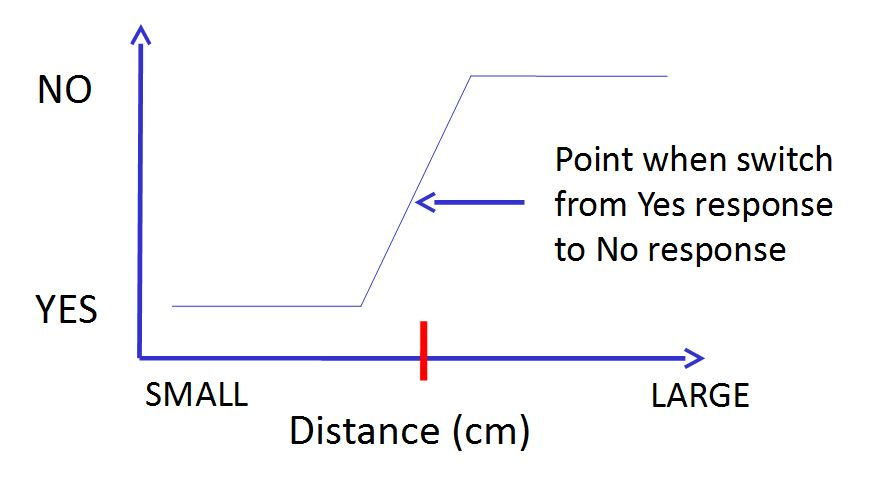
\includegraphics[width=0.75\textwidth]{cross_over}
  \caption{cross over.} 
  \label{fig:cross_over}
\end{figure}

\begin{figure}
\centering
  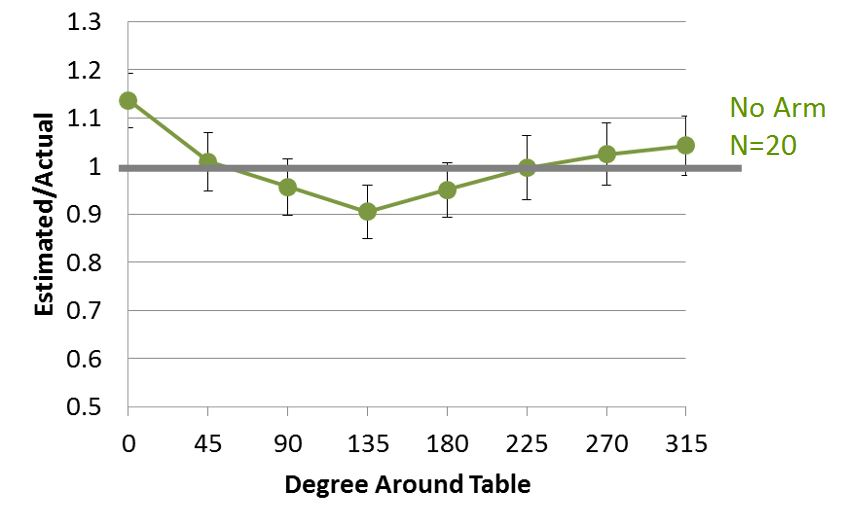
\includegraphics[width=0.75\textwidth]{no_arm_co}
  \caption{no arm co.} 
  \label{fig:no_arm_co}
\end{figure}

\begin{figure}
\centering
  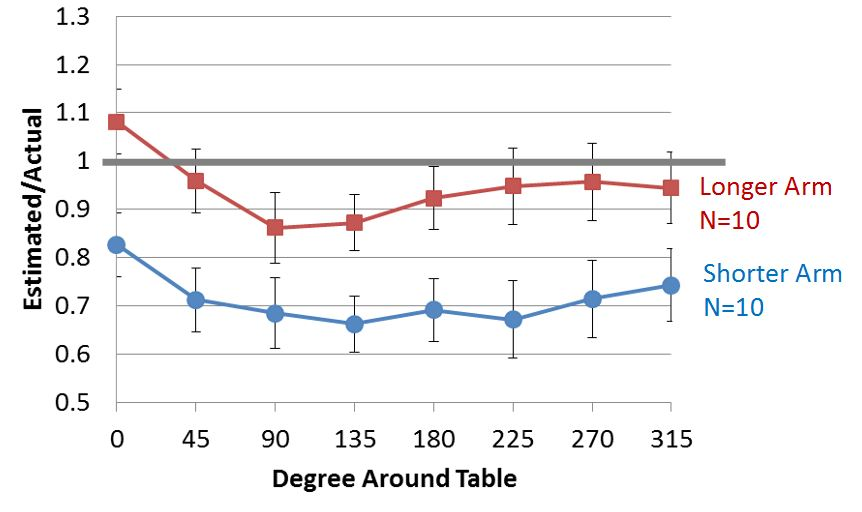
\includegraphics[width=0.75\textwidth]{short_long_arm_co}
  \caption{short long arm co.} 
  \label{fig:short_long_arm_co}
\end{figure}

\begin{figure}
\centering
  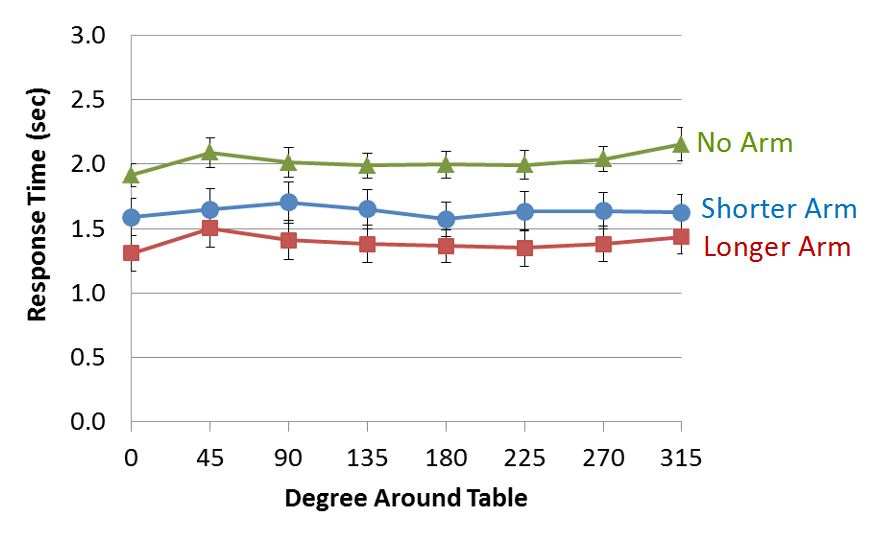
\includegraphics[width=0.75\textwidth]{all_response_time}
  \caption{all response time.} 
  \label{fig:all_response_time}
\end{figure}

\begin{figure}
\centering
  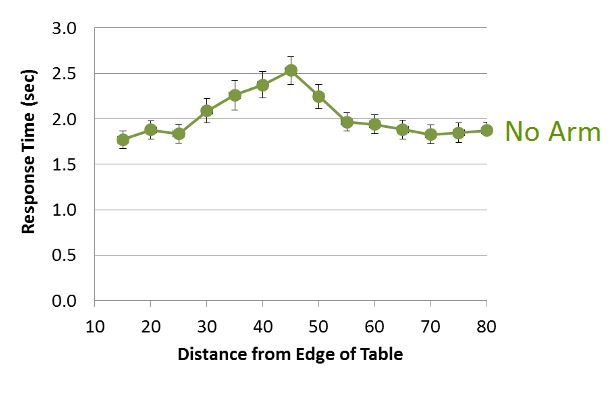
\includegraphics[width=0.75\textwidth]{no_arm_responst_time_dist}
  \caption{all response time.} 
  \label{fig:no_arm_responst_time_dist}
\end{figure}

\begin{figure}
\centering
  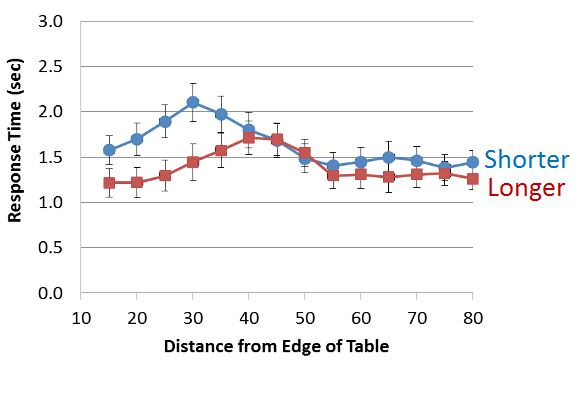
\includegraphics[width=0.75\textwidth]{short_long_arm_responst_time_dist}
  \caption{all response time.} 
  \label{fig:short_long_arm_responst_time_dist}
\end{figure}



Data analysis was done by applying linear mixed models with the Kenward-Rodger degrees of freedom approximation. The random factors were the group number (= an individual number assigned to each group in the group condition), participant number (= an individual number assigned to each individual participant in the single condition) and the number of players(= either one or two). The only fixed factor was the number of players. 

 Although much more data has been recorded during the experiment this section will only cover the most relevant results that suit best to compare the performances of the single vs the group condition. 
 
 All data was automatically recorded from the time participants pressed the controller button to start the task to when they pressed the button again in order to skip to the next task. The data was based on the controller trajectories, rotations and user input.  In the following the term "task duration" will be used to describe the duration in which data was recorded for an individual task.

\subsection{Time to complete}
The time to complete is the average of all task durations.  Figure \ref{fig:results_duration} shows that the groups were much faster with an average of around 50 seconds compared to single participants with an average of around 80 seconds. The output of the linear mixed model was F:(1,18.99) = 52.049, p < 0.001.

\begin{figure}[h]
\centering
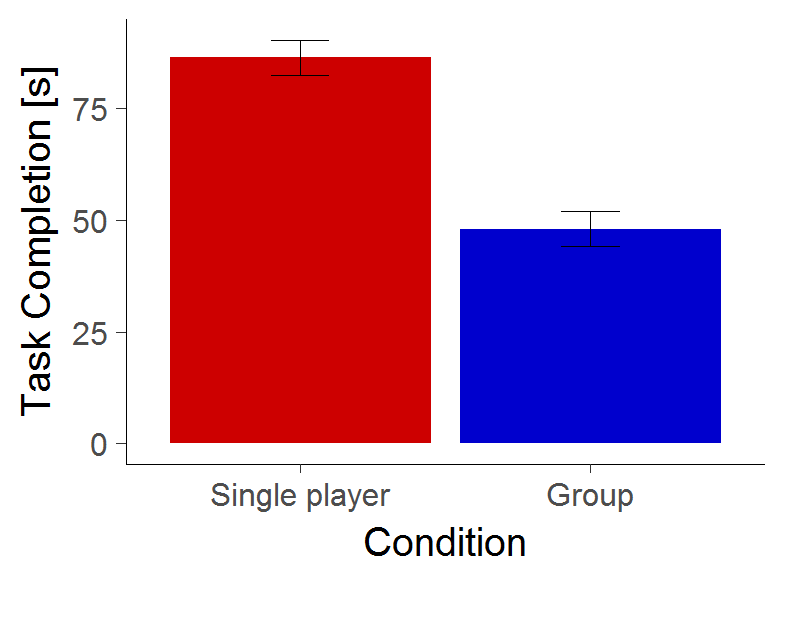
\includegraphics[width=0.5\textwidth]{results_duration}
\caption{Average time to complete in single and group condition.} \label{fig:results_duration}
\end{figure}

\subsection{Rotation sum of cubes}
The rotation sum of cubes is the sum of rotations made by one participant during the task duration. In the group condition we summed up the rotations of both group members first and calculated the averages over the group sums. Figure \ref{fig:results_rotations} shows that the average rotation sum for groups with an average of 5000 degrees was significantly lower compared to single participants with an average of 8000 degrees. For the rotation sum a the smaller value indicates the better performance because the less a participant rotates a cube the more confident and efficient the participant is expected to be at solving the task. The output of the linear mixed model was F:(1,18.99) = 12.164, p < 0.01.

\begin{figure}[h]
\centering
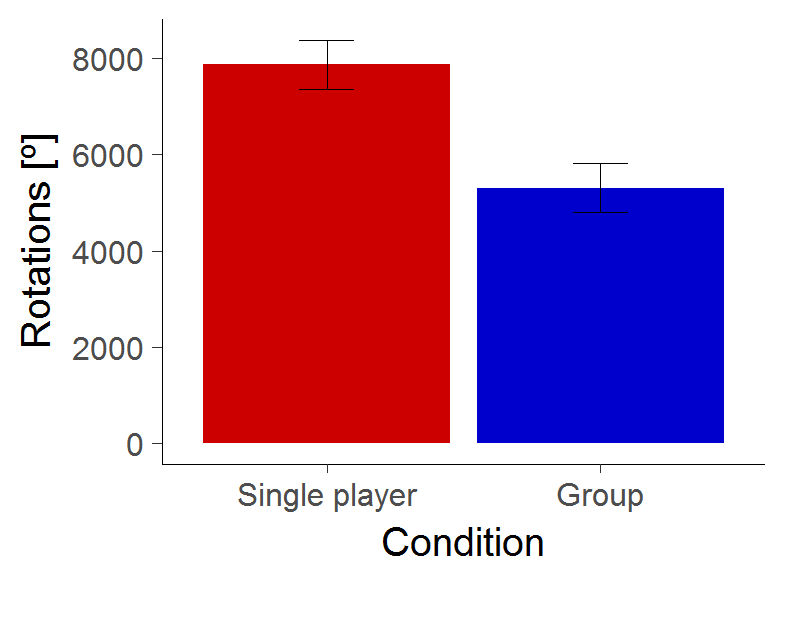
\includegraphics[width=0.5\textwidth]{results_rotations}
\caption{Average sum of rotations in degrees in single and group condition.}
\label{fig:results_rotations}
\end{figure}

\subsection{Number of cube snap-outs}
The number of cube snap-outs is the number of how many times a participant took a cube back out from the problem space during the task duration. Figure \ref{fig:results_snap_outs} shows that groups needed much less snap-outs with an average of 2.1 snap-outs compared to single participants with an average of 4.5 snap-outs. 
Snap-outs can be categorized in two classes: "necessary" and "unnecessary" snap-outs. Necessary snap-outs are the ones which are part of the task design which means participants are supposed to try certain solution paths and if a path was not successful they need to snap-out some cubes and snap-in new ones until they successfully finish the task. It is possible though that participants try the same solution path more than one time and therefore have to do unnecessary snap-outs. For the number of cube snap-outs a smaller value indicates the better performance, because it means that less unnecessary snap-out were made. The average of necessary snap-outs is expected to be equally distributed with an expectancy value of 2.0. In other words scoring an average of 2.0 snap-outs is an indicator of almost "perfect" performance. In the group condition the performance is very close to perfect with an average od 2.1 snap-outs.
The output of the linear mixed model was F:(1,18.99)=22.112, p < 0.001.

\begin{figure}[h]
\centering
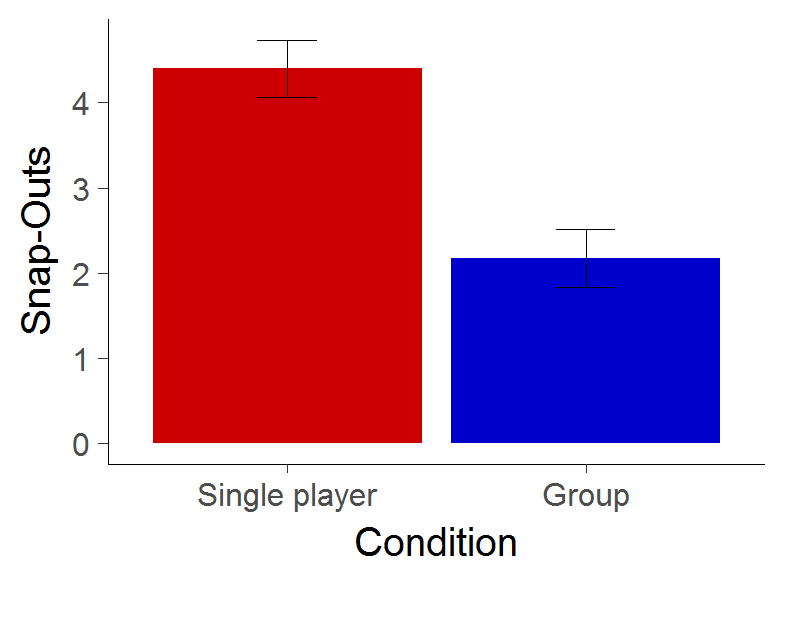
\includegraphics[width=0.5\textwidth]{results_snap_outs}
\caption{Average number of cube snap-outs in single and group condition.}
\label{fig:results_snap_outs}
\end{figure}

\newpage